\section{Métodos de clasificación}

\subsection{Clasificación}
\begin{frame}{\secname : \subsecname}
\begin{block}{Concepto de clasificación}
  Clasificar es convertir valores espectrales en clases de información.
\end{block}
\end{frame}
%--- Next Frame ---%

\begin{frame}{\secname : \subsecname}
\begin{block}{Clase de información}
  Una clase de información es la que describe una categoría en el terreno. \pause Nuestro esquema debe ser completo y sin solapamiento.
\end{block}
\pause
\begin{block}{Clase espectral}
  Es un conjunto de píxeles con valores similares.
\end{block}
\end{frame}
%--- Next Frame ---%

\begin{frame}{\secname : \subsecname}
  \begin{table}[hbt]
      \centering
      \begin{tabular}{p{12cm}c}
          \toprule
          Nombre & Color \\
          \midrule
          Áreas terrestres cultivadas y manejada & \textcolor{A11}{$\blacksquare$}\texttt{\#b2df8a}
          \\
          Vegetación natural y semi-natural  & \textcolor{A12}{$\blacksquare$}\texttt{\#33a02c}\\
          Áreas acuáticas o regularmente inundadas cultivadas &
          \textcolor{A23}{$\blacksquare$}\texttt{\#fdbf6f}\\
          Vegetación natural y semi-natural acuática o
  	regularmente inundadas  & \textcolor{A24}{$\blacksquare$}\texttt{\#ff7f00}\\
          Superficies artificiales y áreas asociadas  &
          \textcolor{B15}{$\blacksquare$}\texttt{\#fb9a99}\\
          Áreas descubiertas o desnudas  & \textcolor{B16}{$\blacksquare$}\texttt{\#e31a1c}\\
          Cuerpos artificiales de agua, nieve y hielo  &
          \textcolor{B27}{$\blacksquare$}\texttt{\#a6cee3}\\
          Cuerpos naturales de agua, nieve y hielo &
          \textcolor{B28}{$\blacksquare$}\texttt{\#1f78b4}\\
          \bottomrule
      \end{tabular}
  \caption{\label{tab:usos}Categorias usos del suelo segun el esquema LCCS2 de la FAO.}
  \end{table}
\end{frame}

\begin{frame}{\secname : \subsecname}
  \begin{block}{Esquema general de clasificación}
    \begin{center}
    \smartdiagramset{back arrow disabled=true,text width = 2.6cm,module x sep=3.75cm}
    \smartdiagram[flow diagram:horizontal]{Información espectral, Algorítmo de clasificación, Clases de información}
    \end{center}
  \end{block}
\end{frame}
%--- Next Frame ---%

\begin{frame}{\secname : \subsecname}
  \begin{figure}
    \centering
    \subfloat[Imagen original]{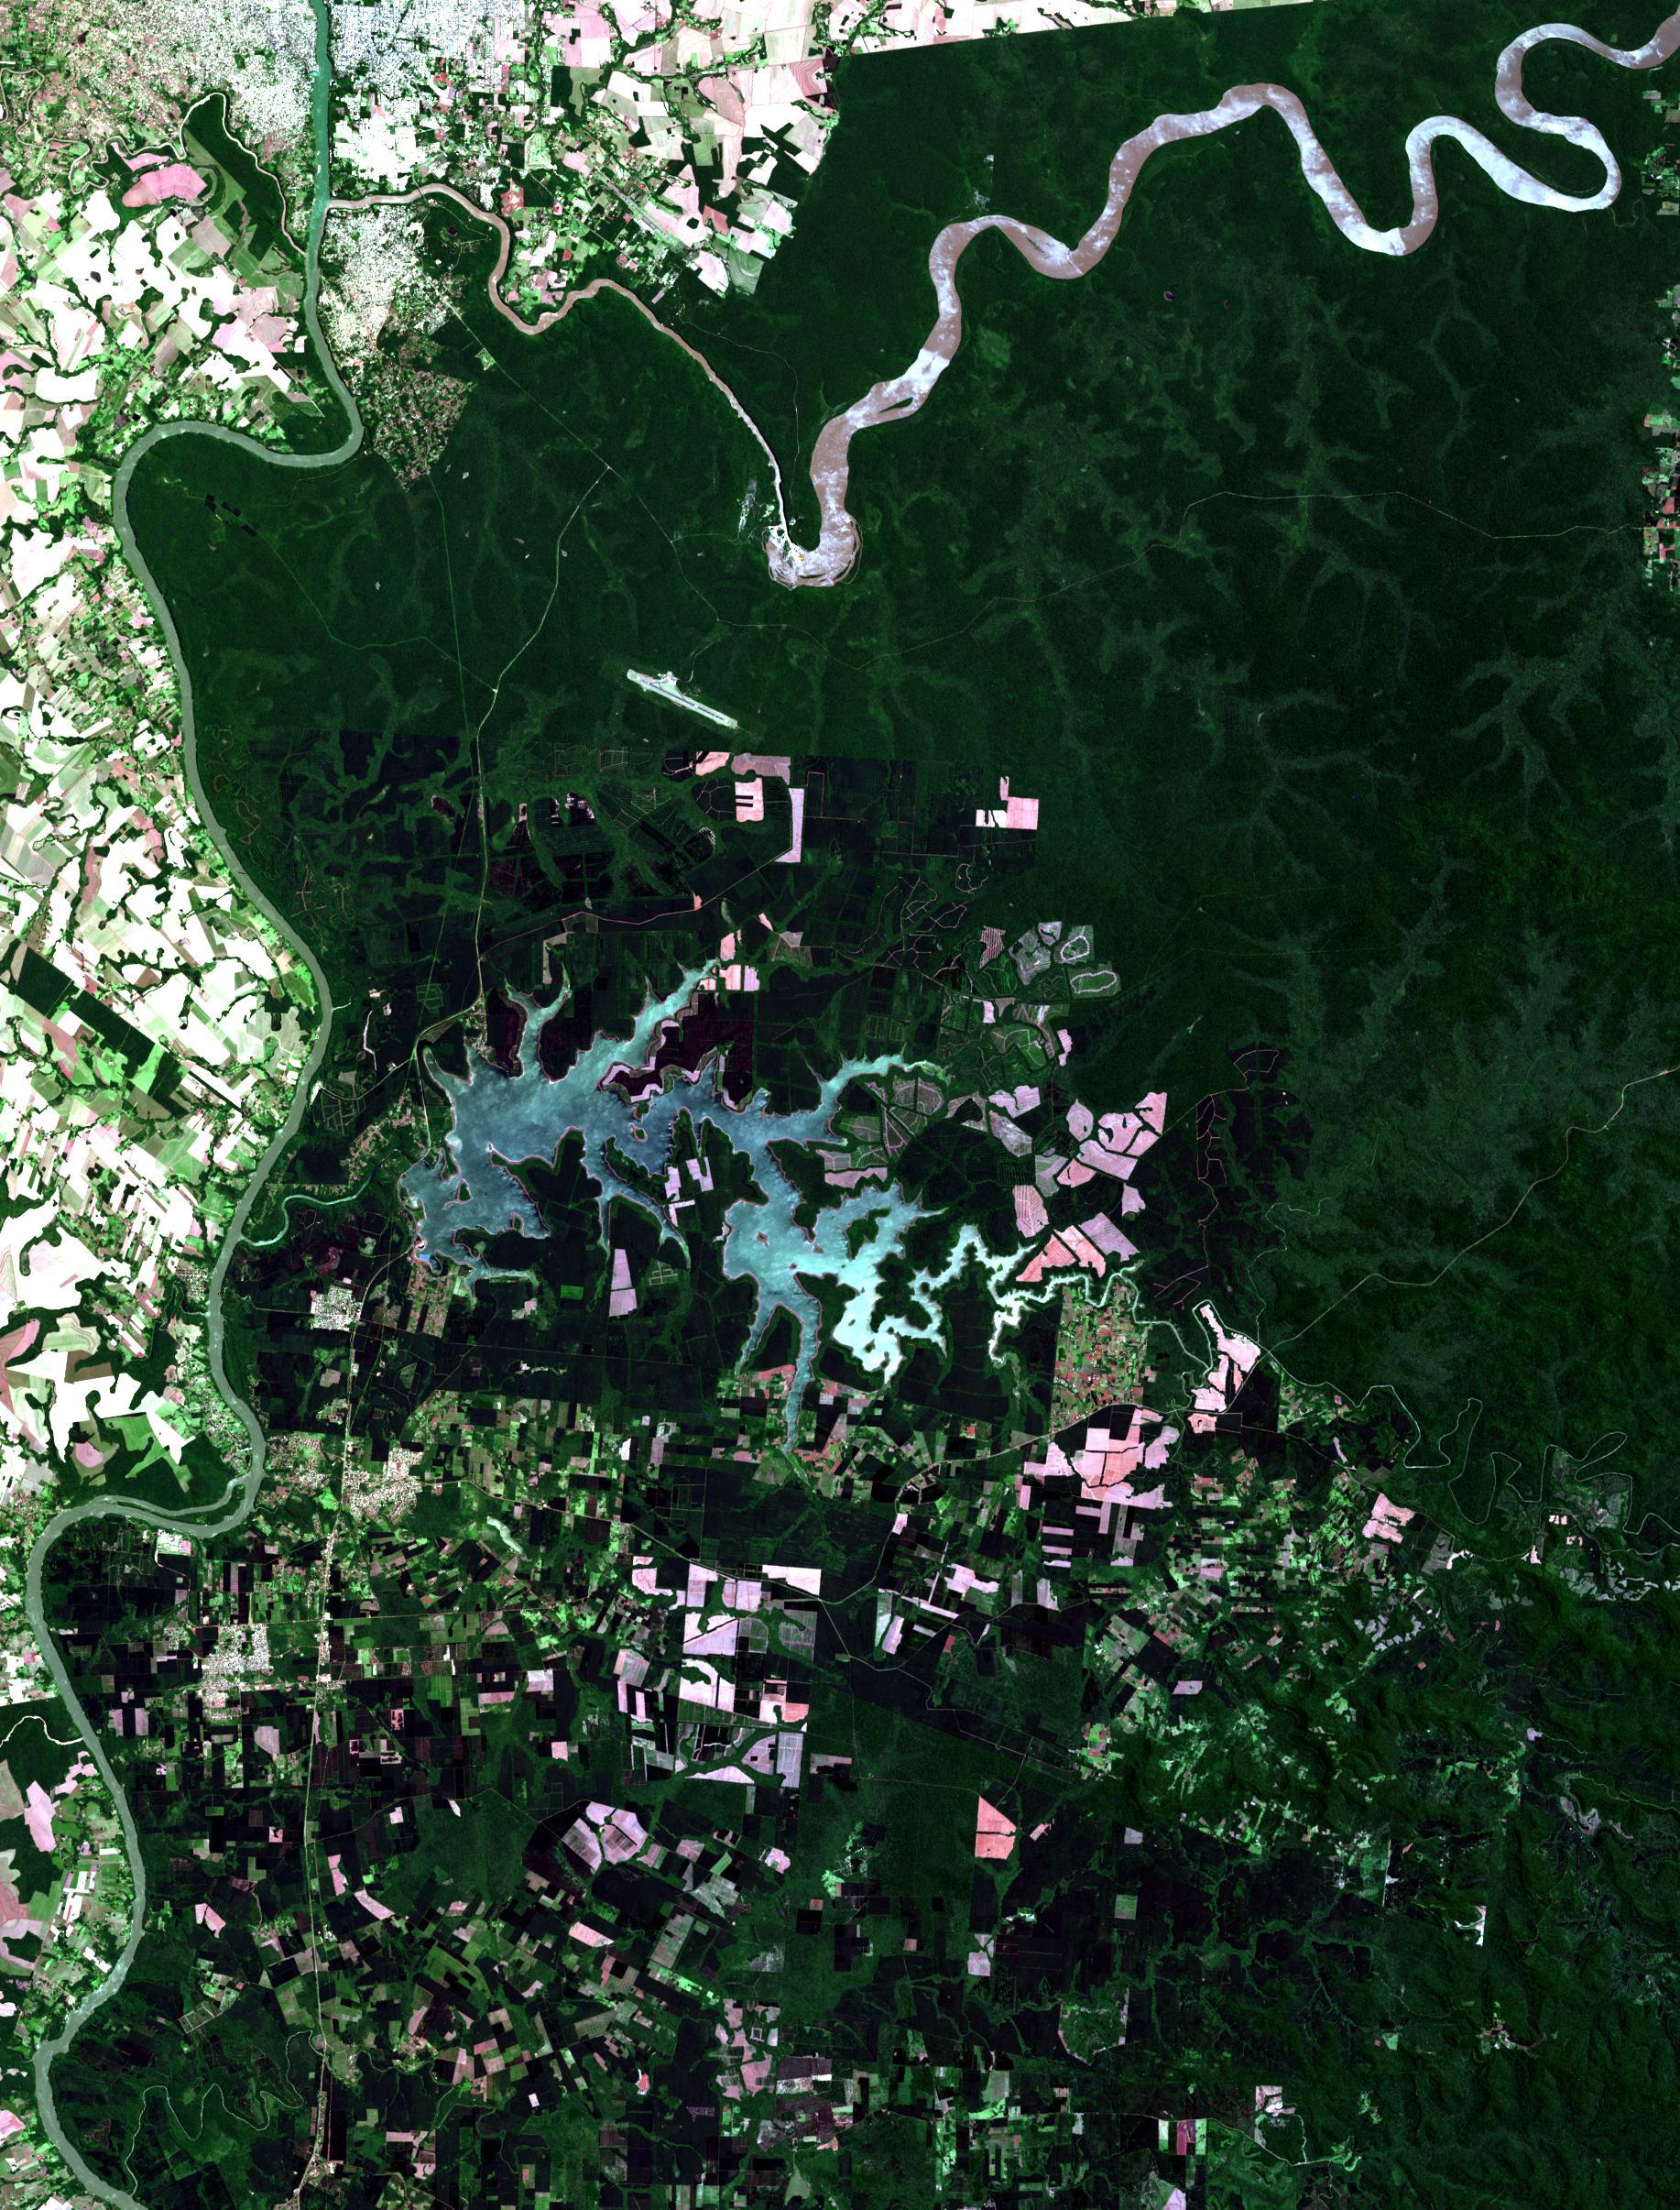
\includegraphics[width=0.3\textwidth]{fig:rgb-class.jpg}}
    \hspace{1cm}
    \subfloat[Imagen clasificada]{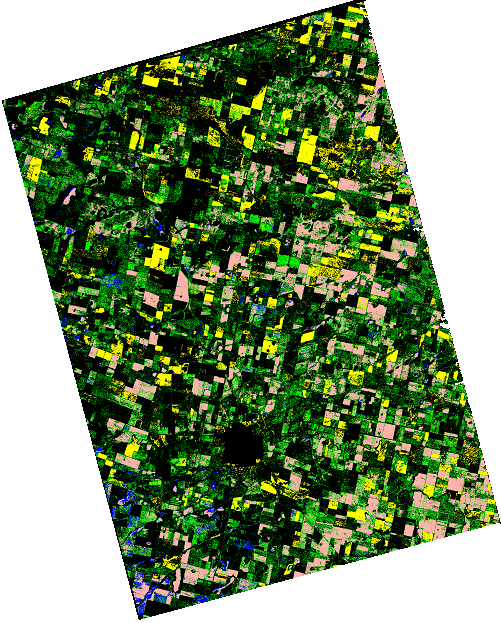
\includegraphics[width=0.3\textwidth]{fig:class} }
    \caption{Clasificación de una imagen Landsat 8 de la zona de triple frontera.}
    \label{}
  \end{figure}
\end{frame}
%--- Next Frame ---%

\subsection{Métodos supervisados}
\begin{frame}{\secname : \subsecname}
    \begin{center}
      \smartdiagramset{back arrow disabled=true,text width = 2.6cm,module x sep=3.75cm,
      additions={
            additional item offset=0.5cm,
            additional item border color=red,
            additional connections disabled=false,
            additional arrow color=red,
            additional arrow tip=stealth,
            additional arrow line width=1pt,
            additional item width=3cm,
            additional item text width=3cm,
        }}
      \smartdiagramadd[flow diagram:horizontal]{Áreas de entrenamiento, Algorítmo de clasificación, Clases de información}
      {above of module1/Información espectral,below of module1/Información del terreno}
    \end{center}
\end{frame}
%--- Next Frame ---%


\subsection{Clustering}
\begin{frame}{\secname : \subsecname}
  \begin{center}
  \smartdiagramset{back arrow disabled=true,text width = 2.6cm,module x sep=3.75cm,
  additions={
        additional item offset=0.5cm,
        additional item border color=red,
        additional connections disabled=false,
        additional arrow color=red,
        additional arrow tip=stealth,
        additional arrow line width=1pt,
        additional item width=3cm,
        additional item text width=3cm,
    }}
  \smartdiagramadd[flow diagram:horizontal]{Algorítmo de clasificación, Clases espectrales, Clases de información}
  {above of module1/Información espectral,below of module2/Información del terreno}
  \end{center}
\end{frame}
%--- Next Frame ---%

\subsection{k-means}

\begin{frame}{\secname : \subsecname}
  \begin{figure}
    \centering
    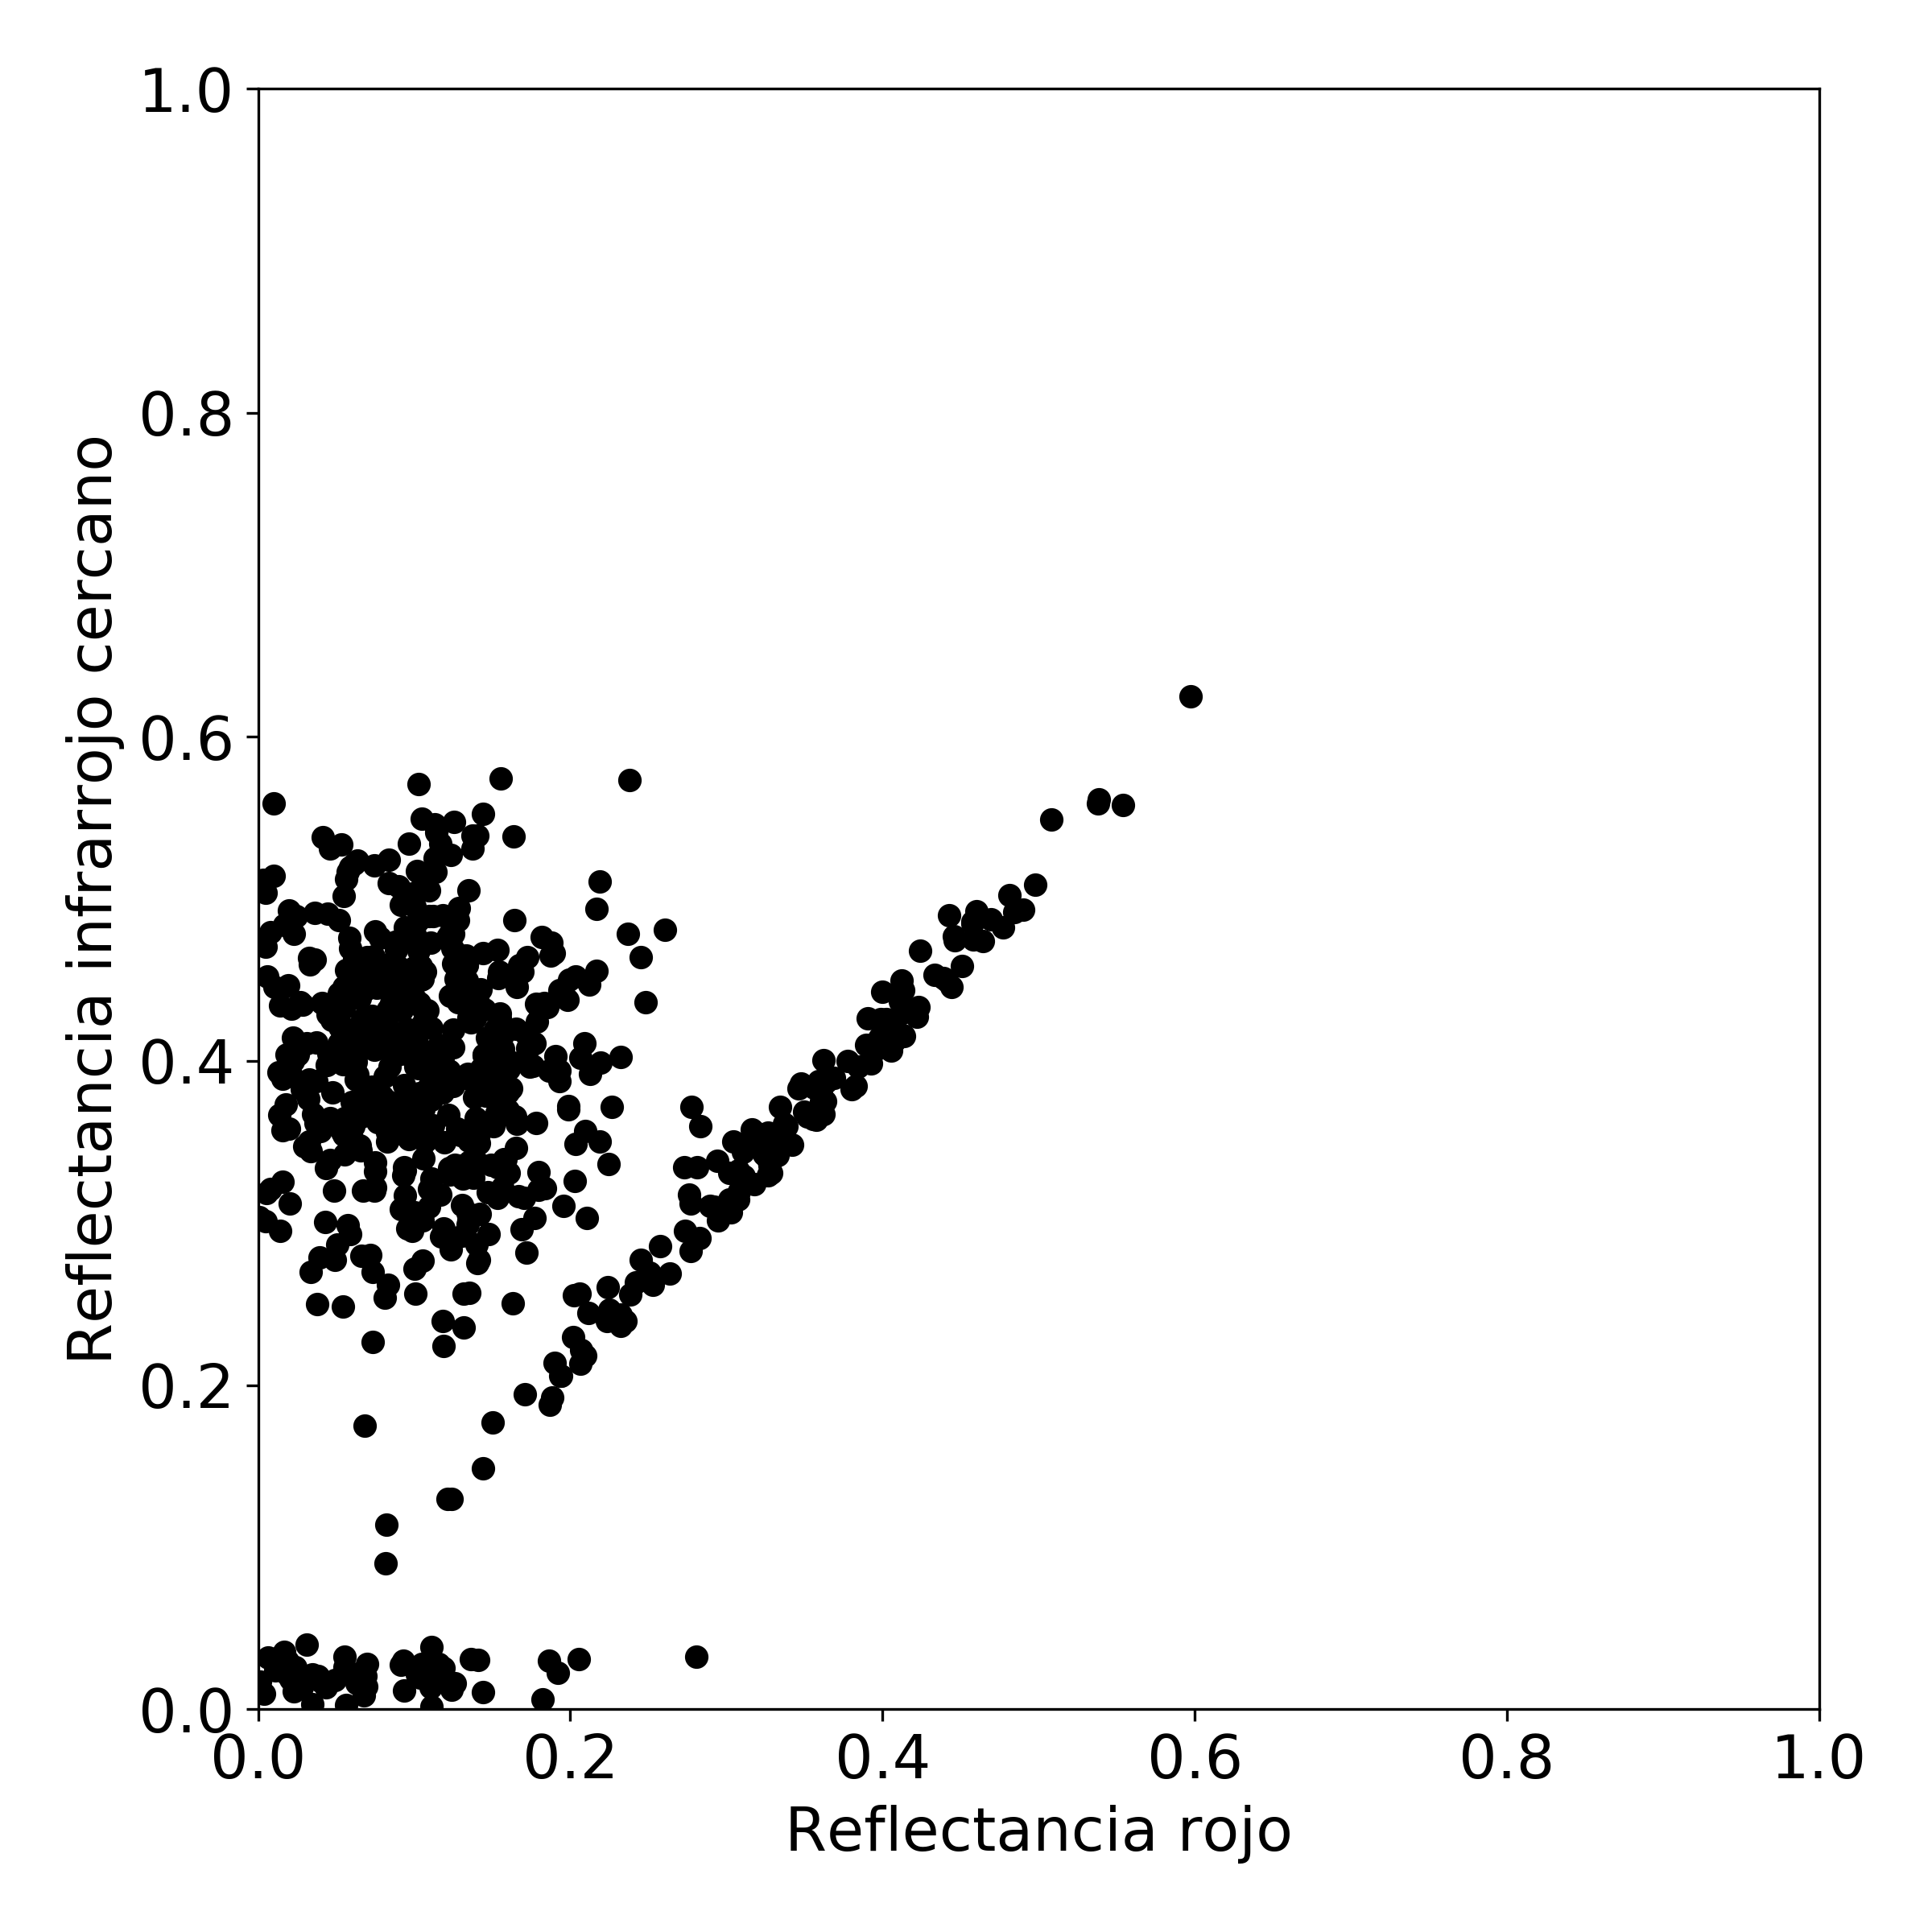
\includegraphics[width=0.4\textwidth]{fig:cluster-black}
    \caption{Clasificación por kmeans.}
    \label{}
  \end{figure}
\end{frame}
%--- Next Frame ---%

\begin{frame}{\secname : \subsecname}
  \begin{figure}
    \centering
    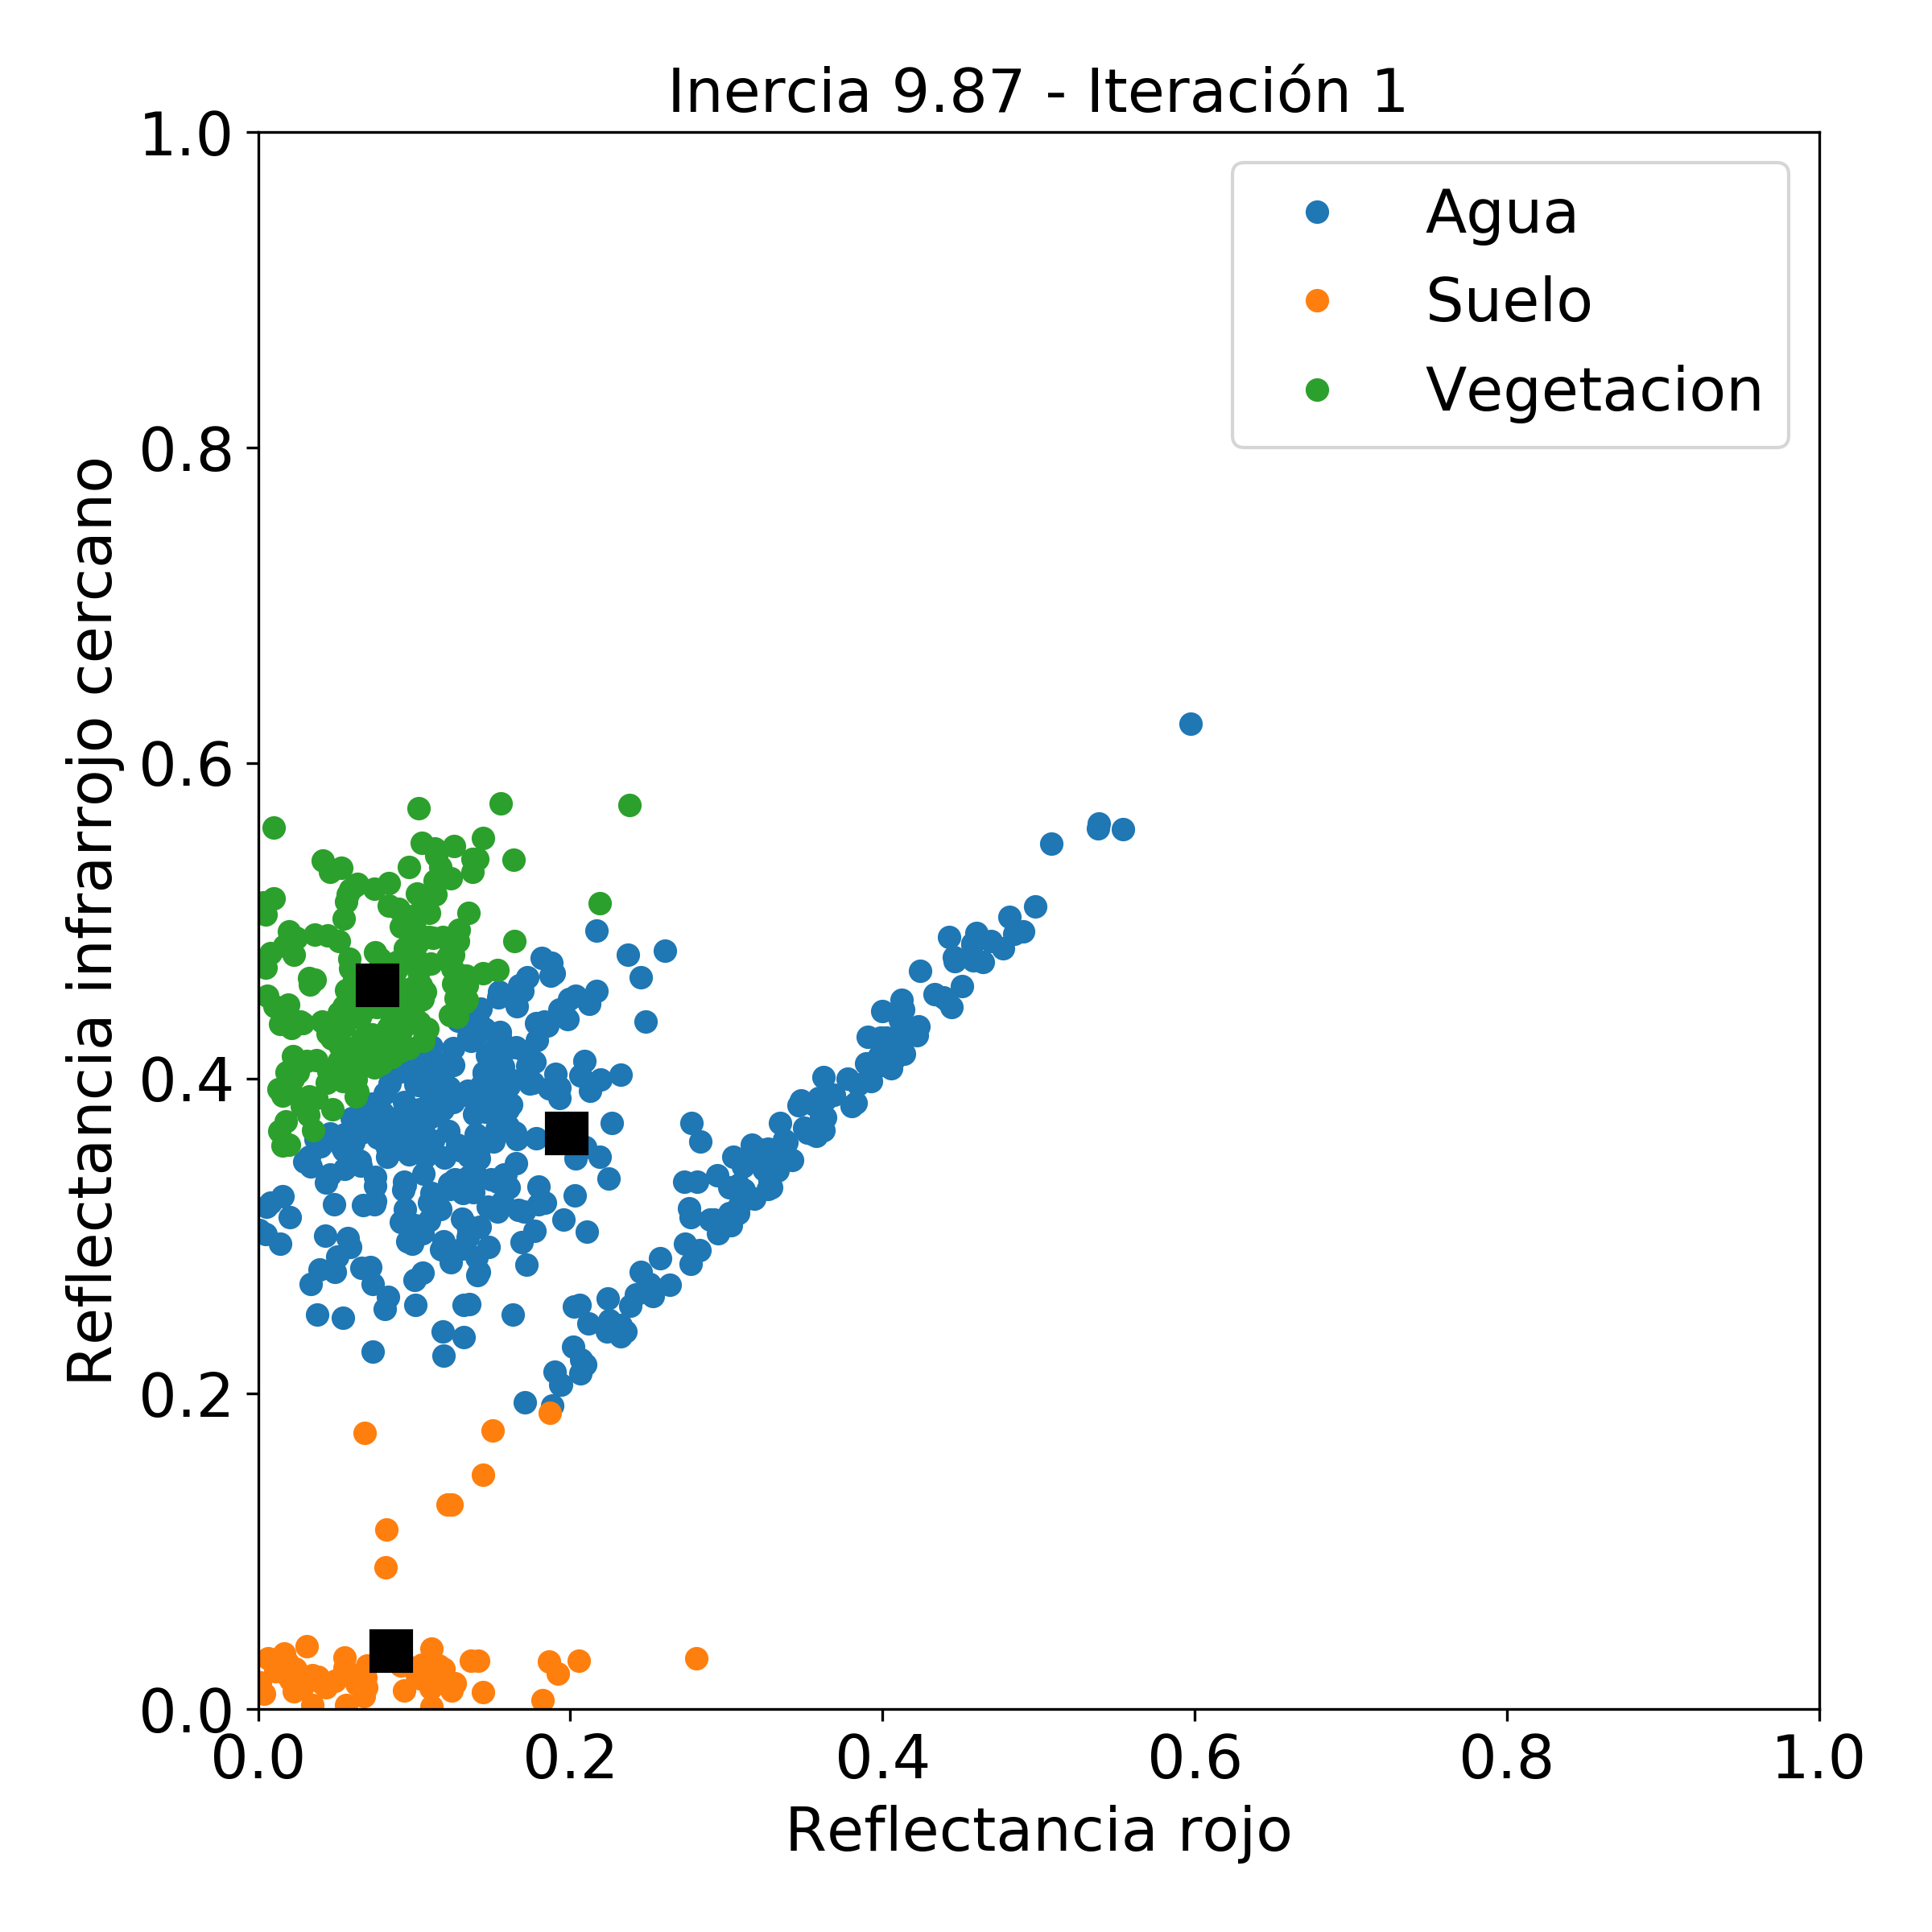
\includegraphics[width=0.4\textwidth]{fig:cluster-1}
    \caption{Clasificación por kmeans.}
    \label{}
  \end{figure}
\end{frame}
%--- Next Frame ---%

\begin{frame}{\secname : \subsecname}
  \begin{figure}
    \centering
    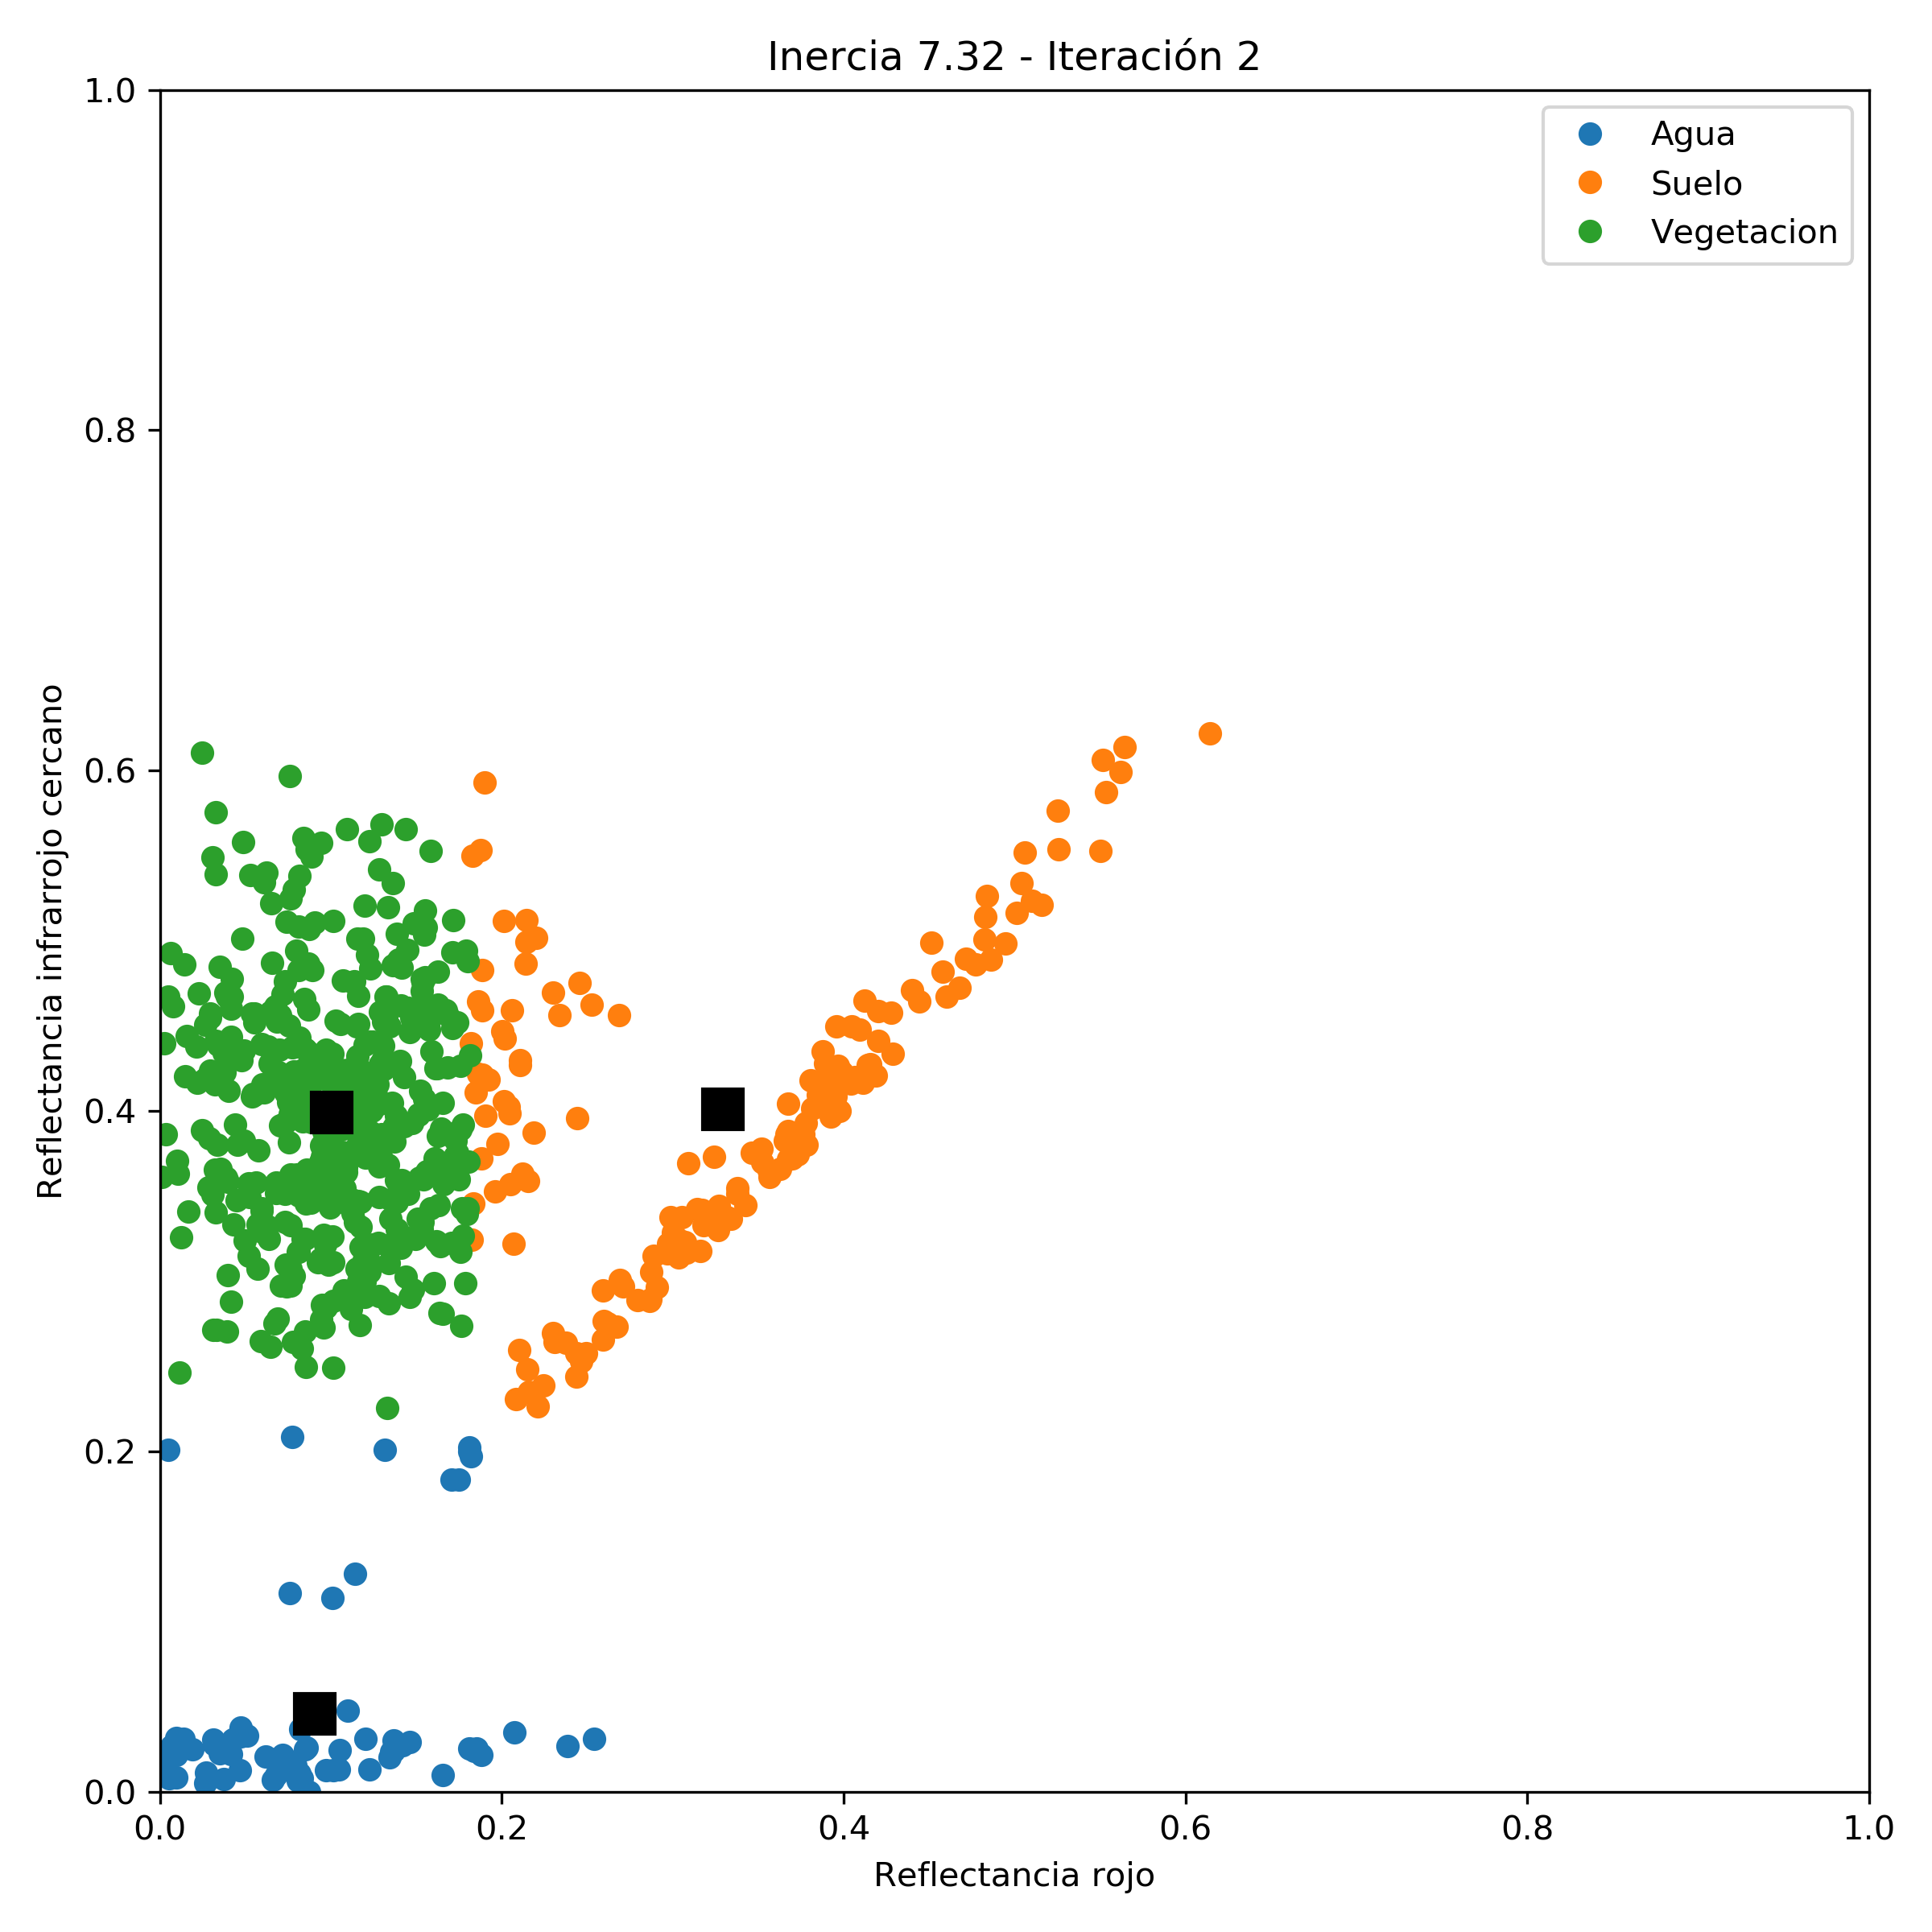
\includegraphics[width=0.4\textwidth]{fig:cluster-2}
    \caption{Clasificación por kmeans.}
    \label{}
  \end{figure}
\end{frame}
%--- Next Frame ---%

\begin{frame}{\secname : \subsecname}
  \begin{figure}
    \centering
    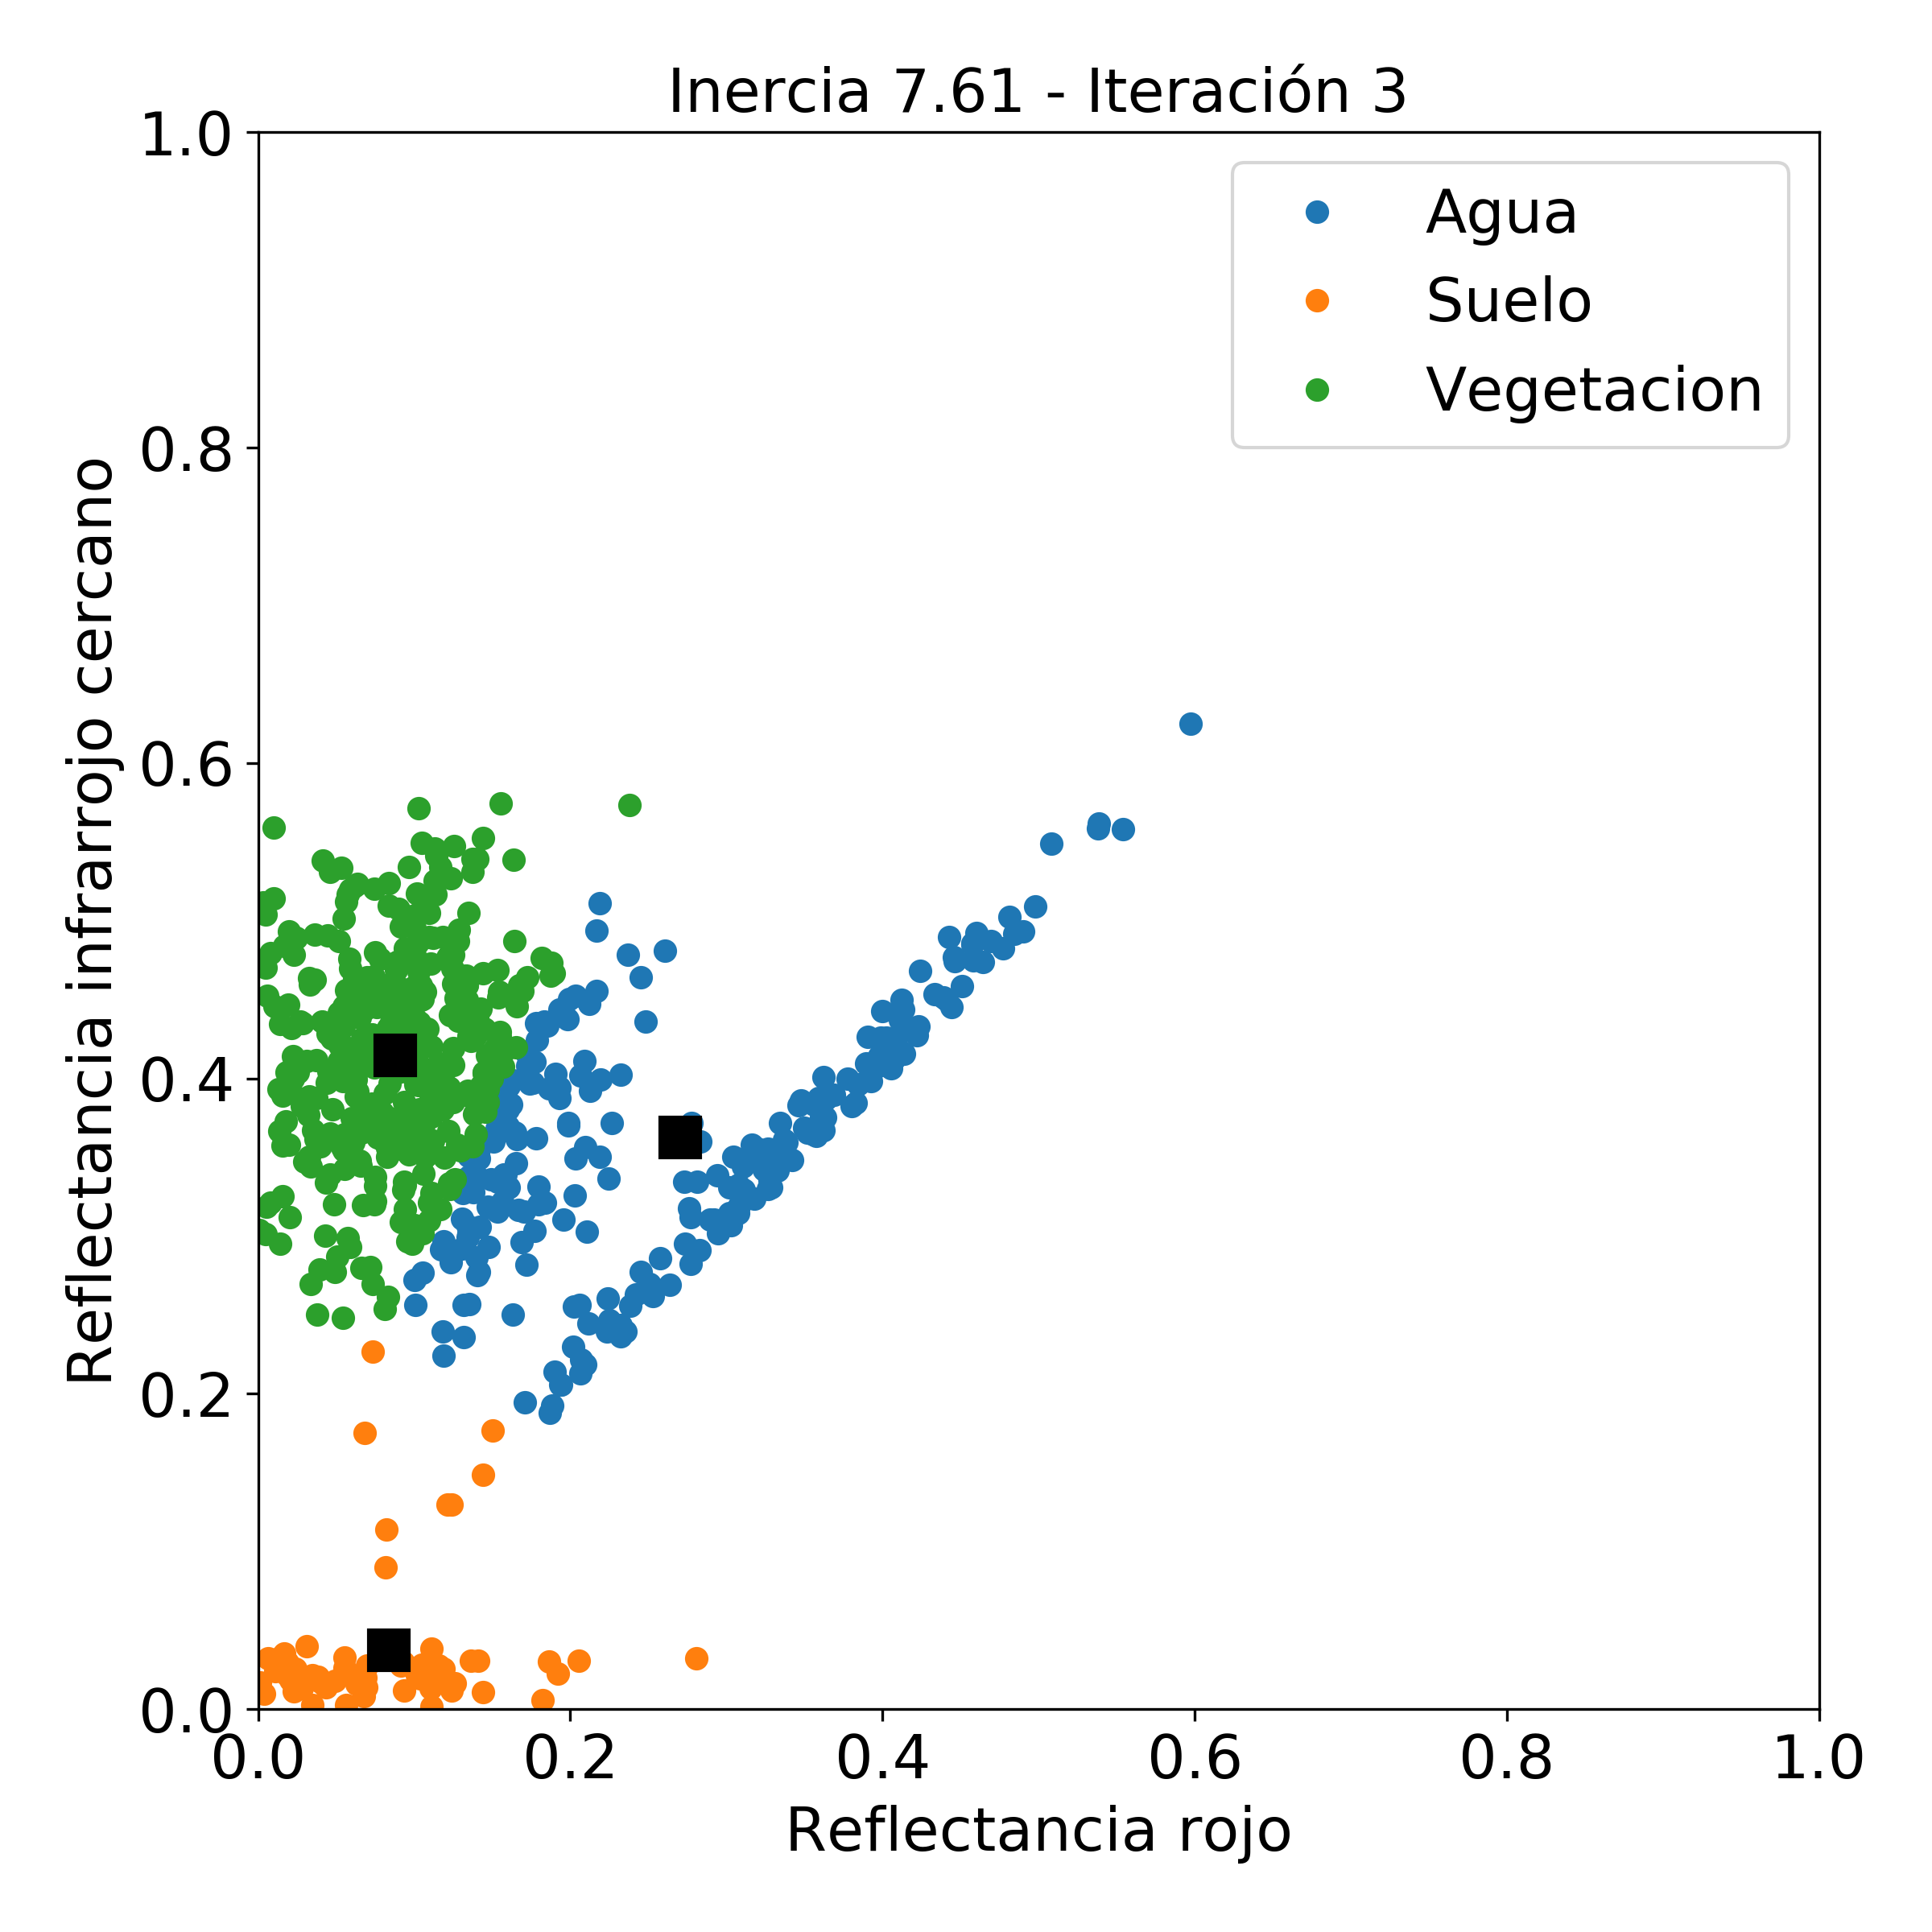
\includegraphics[width=0.4\textwidth]{fig:cluster-3}
    \caption{Clasificación por kmeans.}
    \label{}
  \end{figure}
\end{frame}
%--- Next Frame ---%

\begin{frame}{\secname : \subsecname}
  \begin{figure}
    \centering
    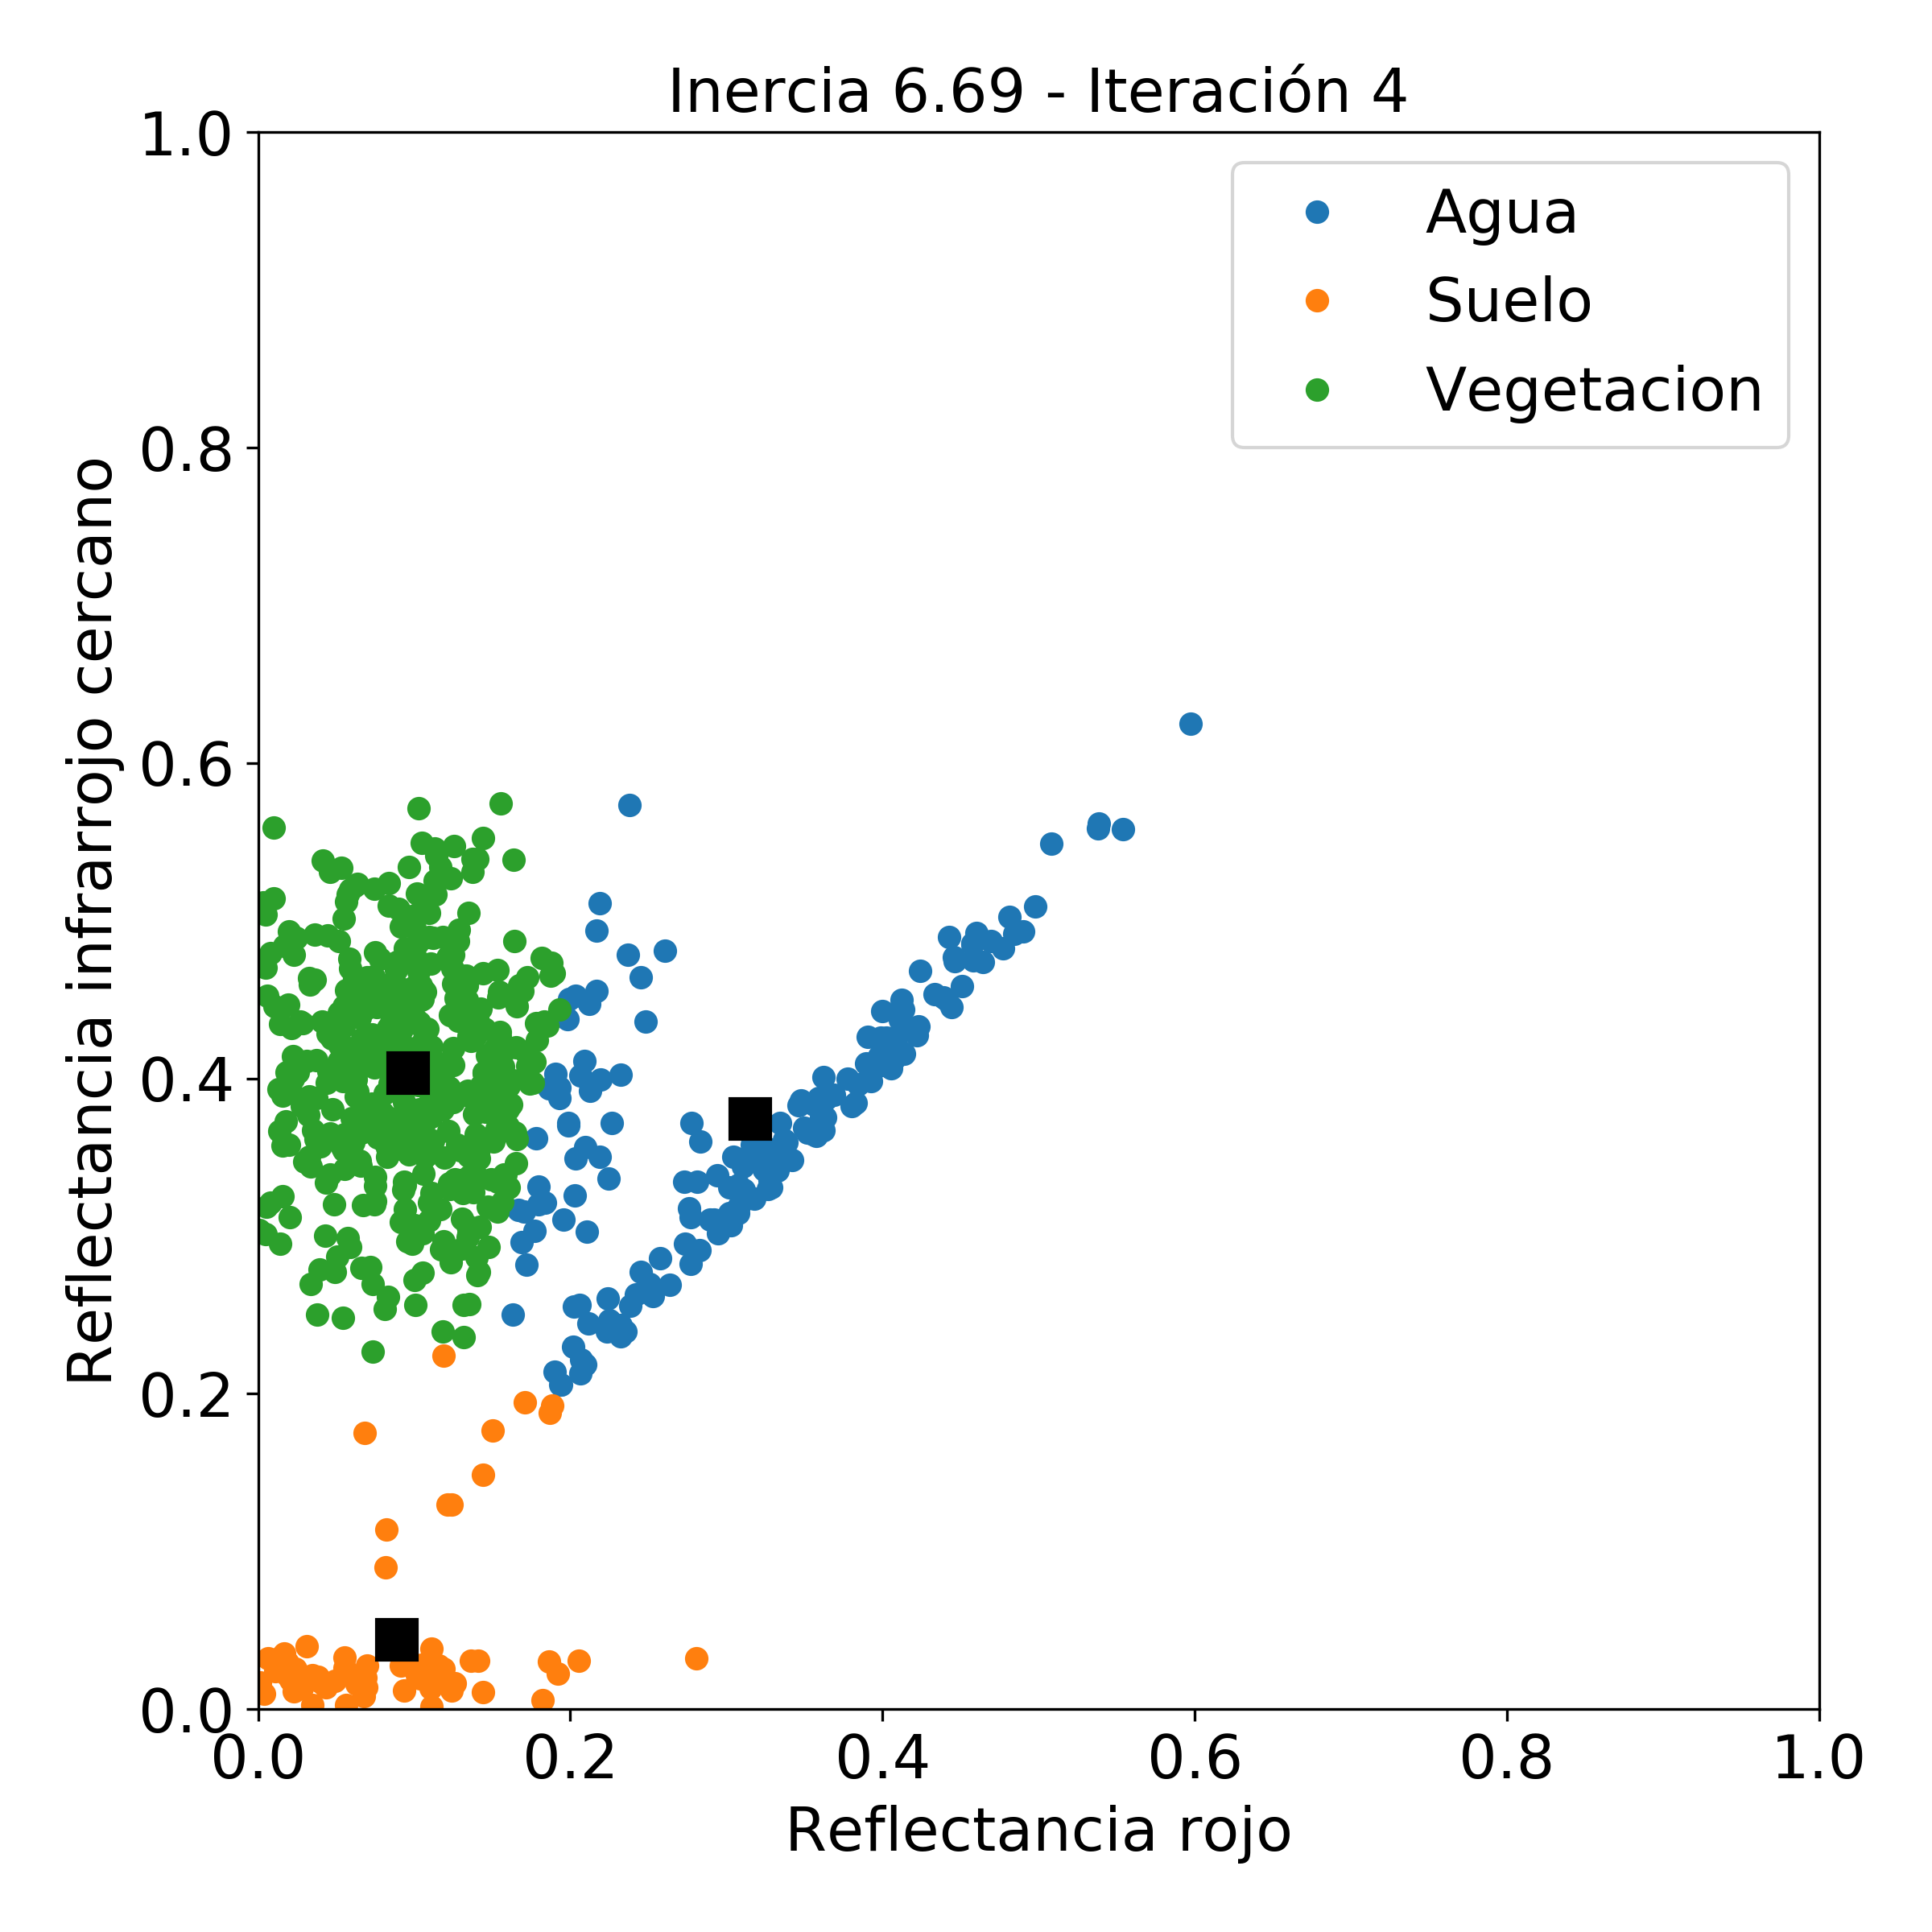
\includegraphics[width=0.4\textwidth]{fig:cluster-4}
    \caption{Clasificación por kmeans.}
    \label{}
  \end{figure}
\end{frame}
%--- Next Frame ---%

\begin{frame}{\secname : \subsecname}
  \begin{figure}
    \centering
    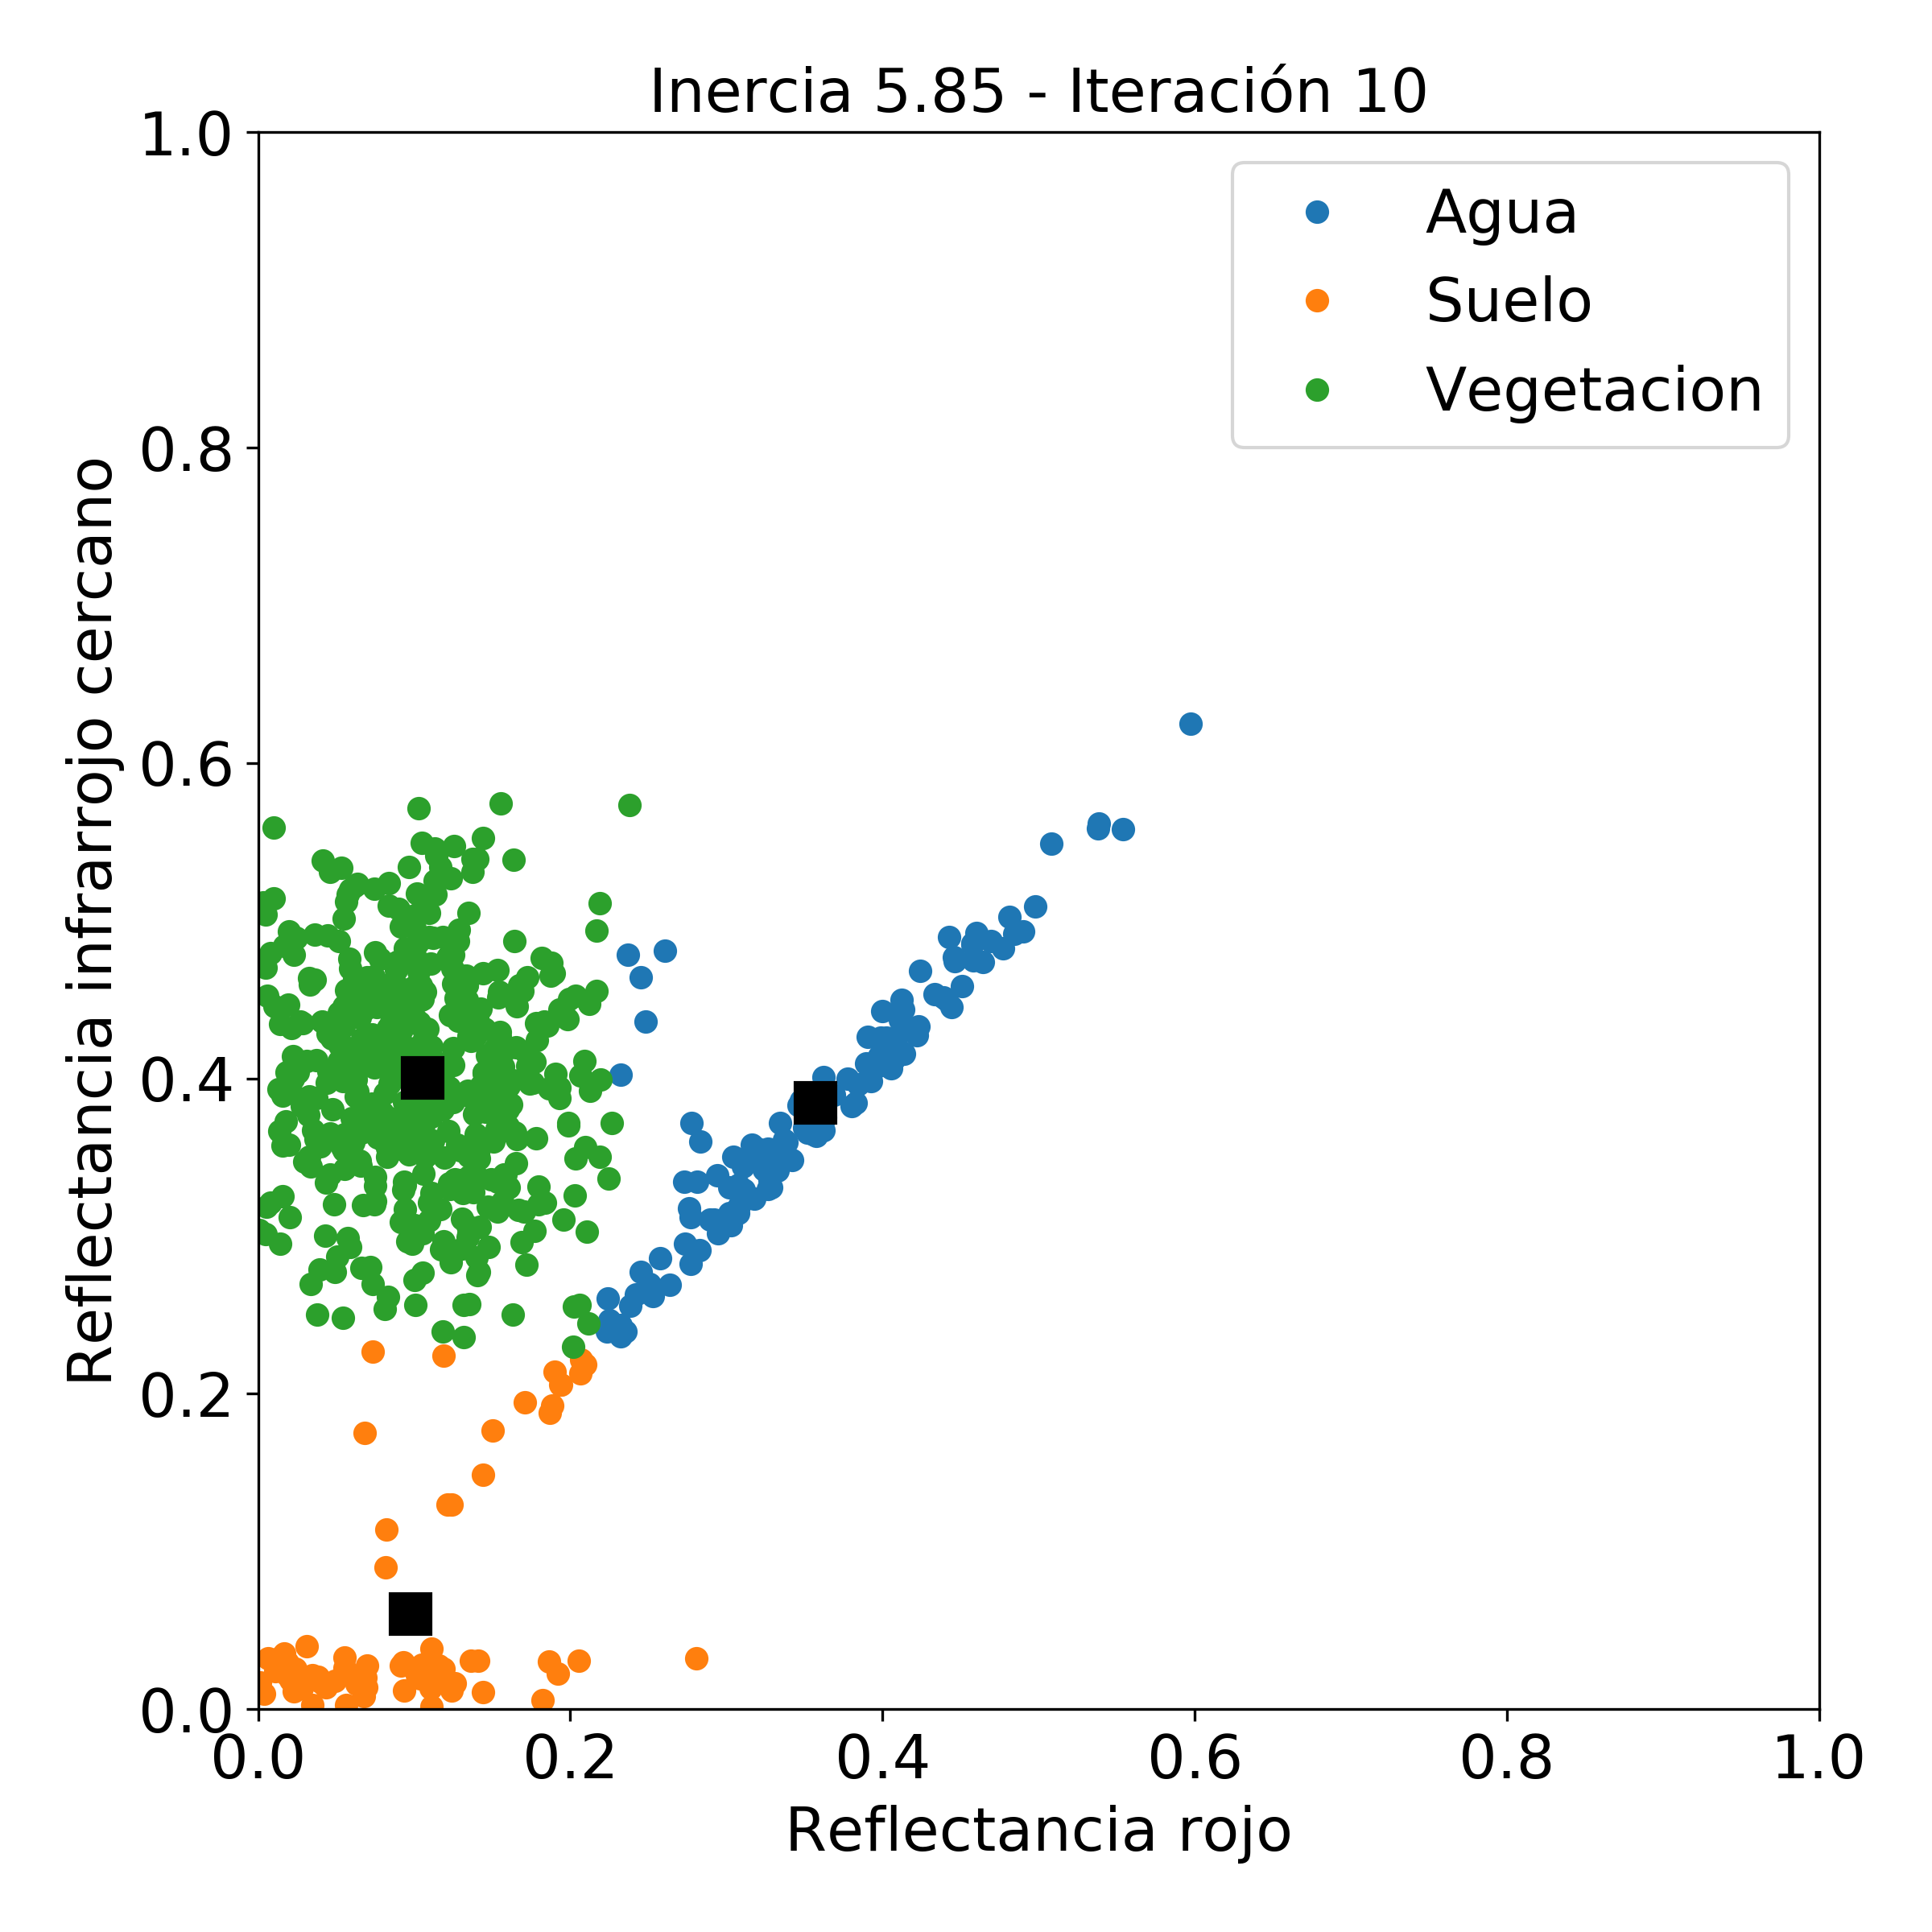
\includegraphics[width=0.4\textwidth]{fig:cluster-10}
    \caption{Clasificación por kmeans.}
    \label{}
  \end{figure}
\end{frame}
%--- Next Frame ---%

\begin{frame}{\secname : \subsecname}
  \begin{figure}
    \centering
    \subfloat[Clases de información]{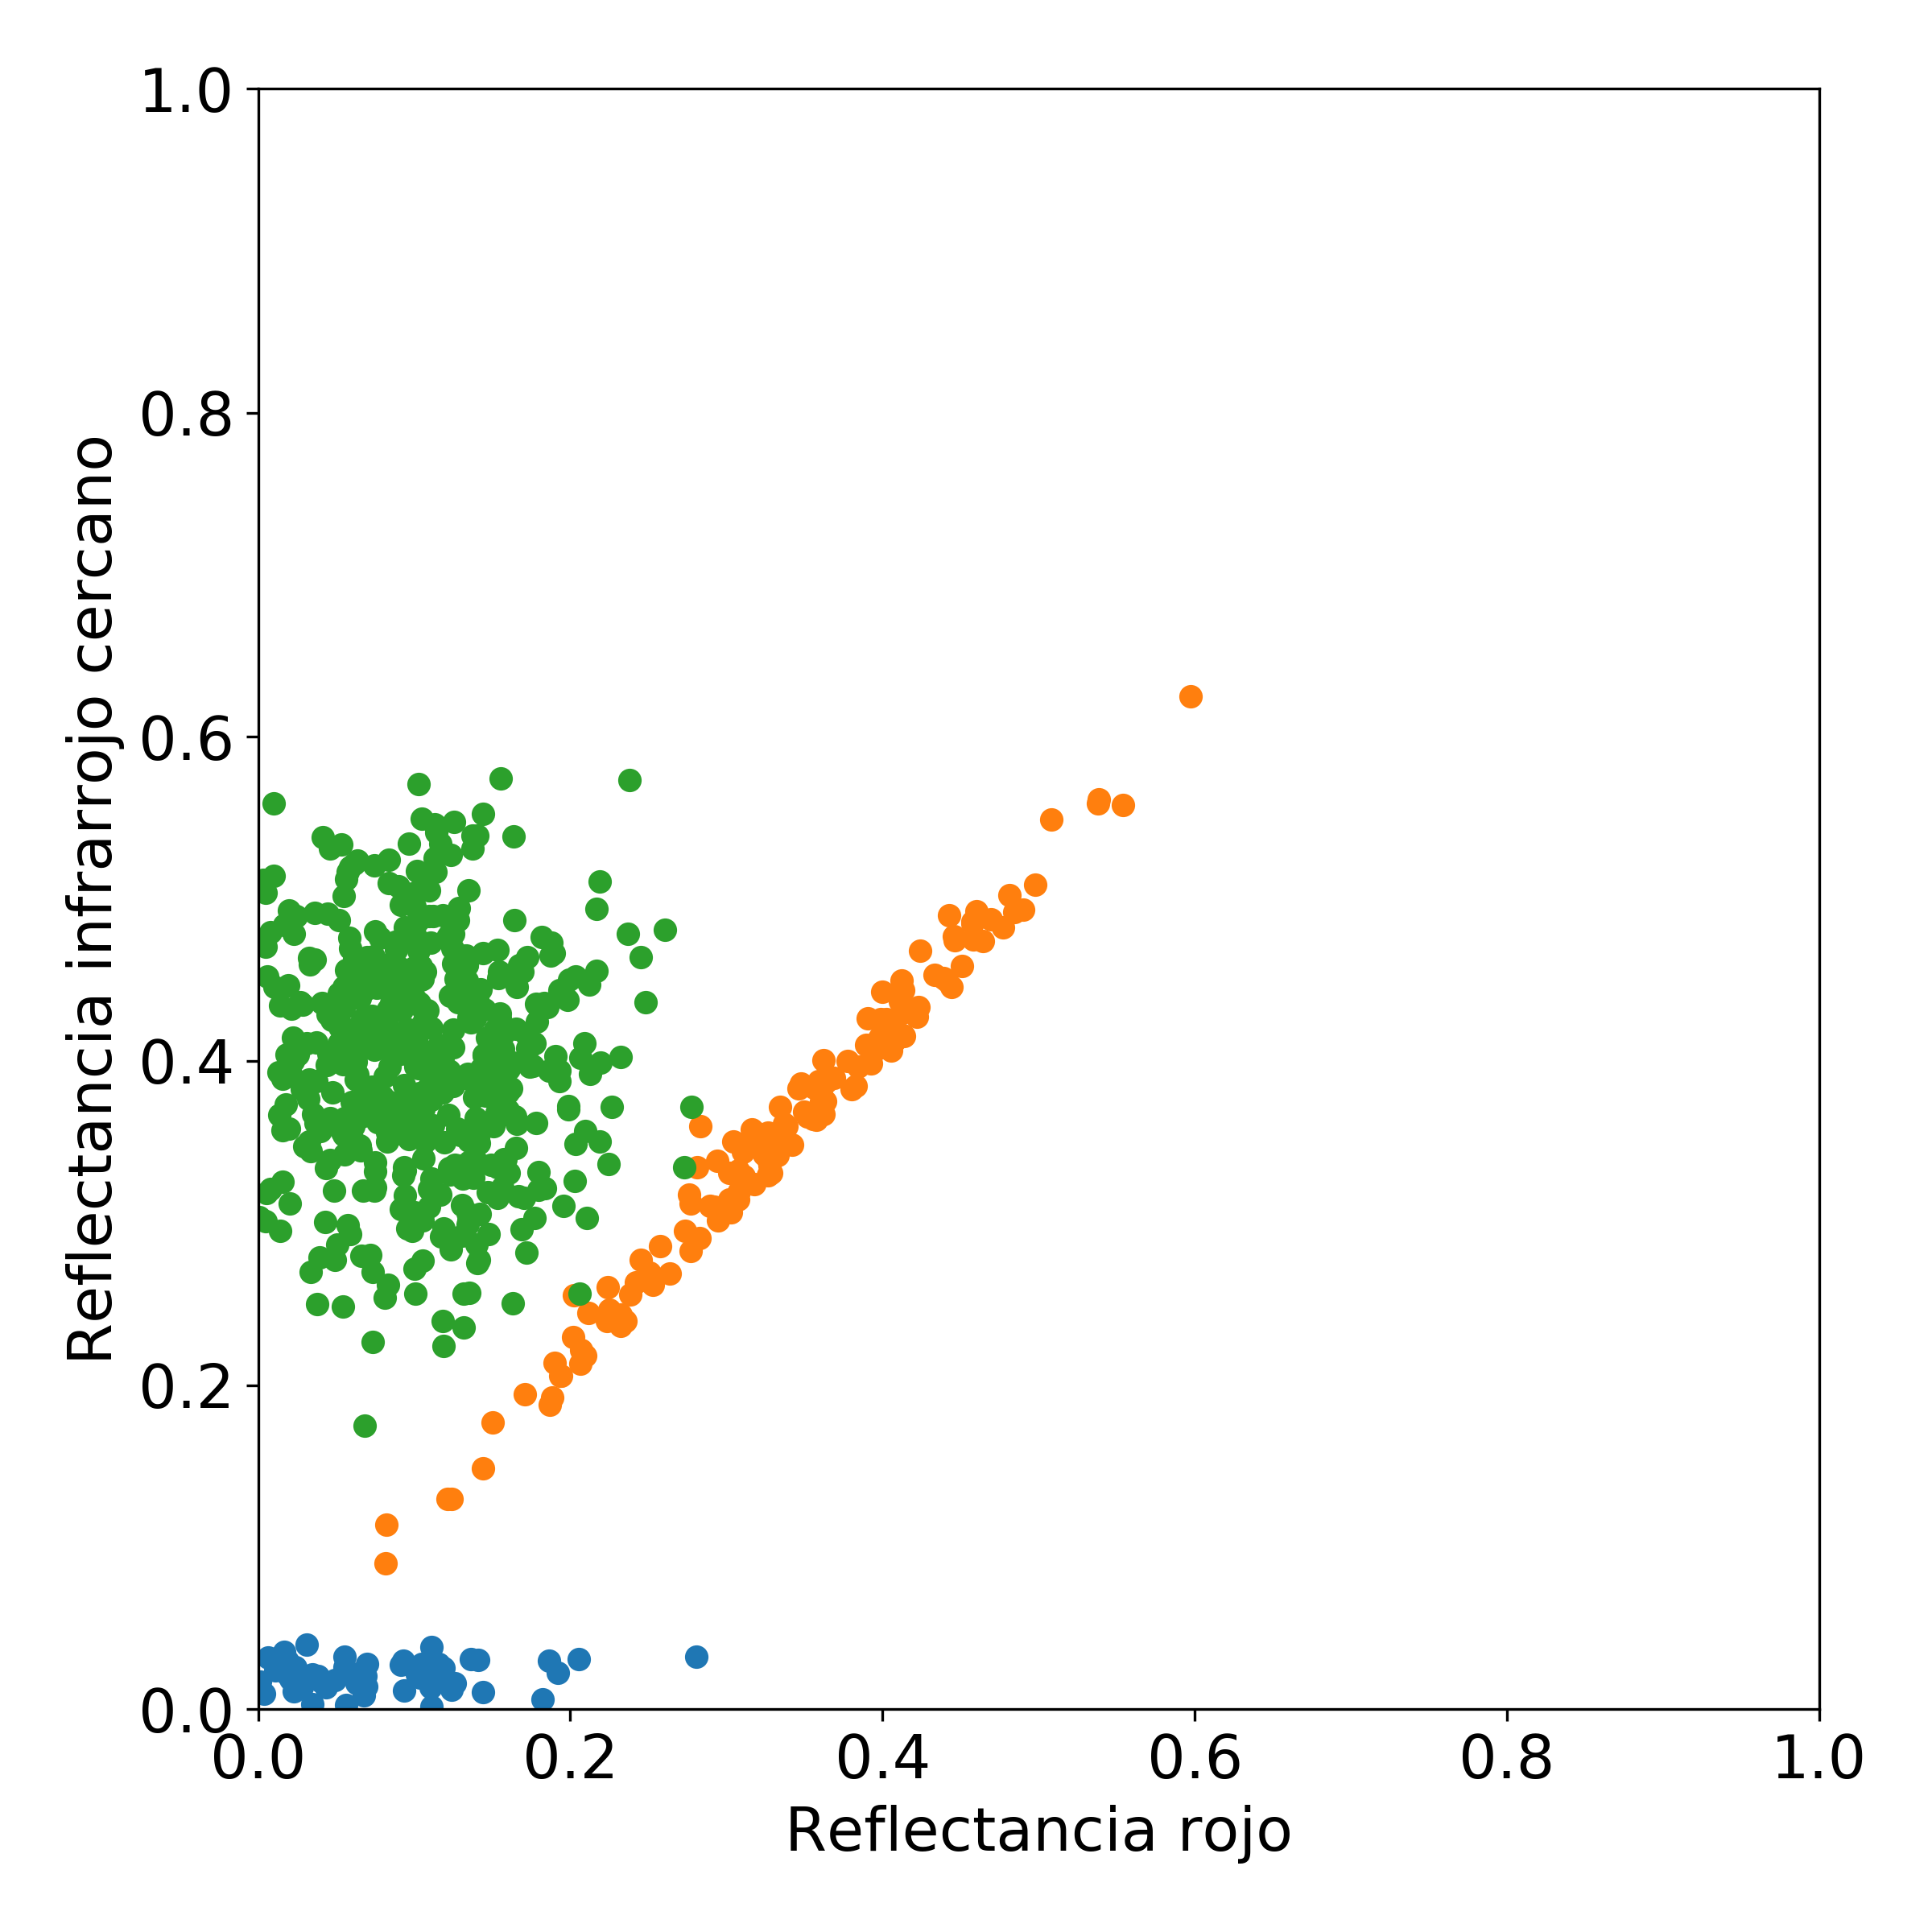
\includegraphics[width=0.4\textwidth]{fig:cluster-info}\label{fig:kmeans2}}
    \hspace{1cm}
    \subfloat[Clasificación obtenida]{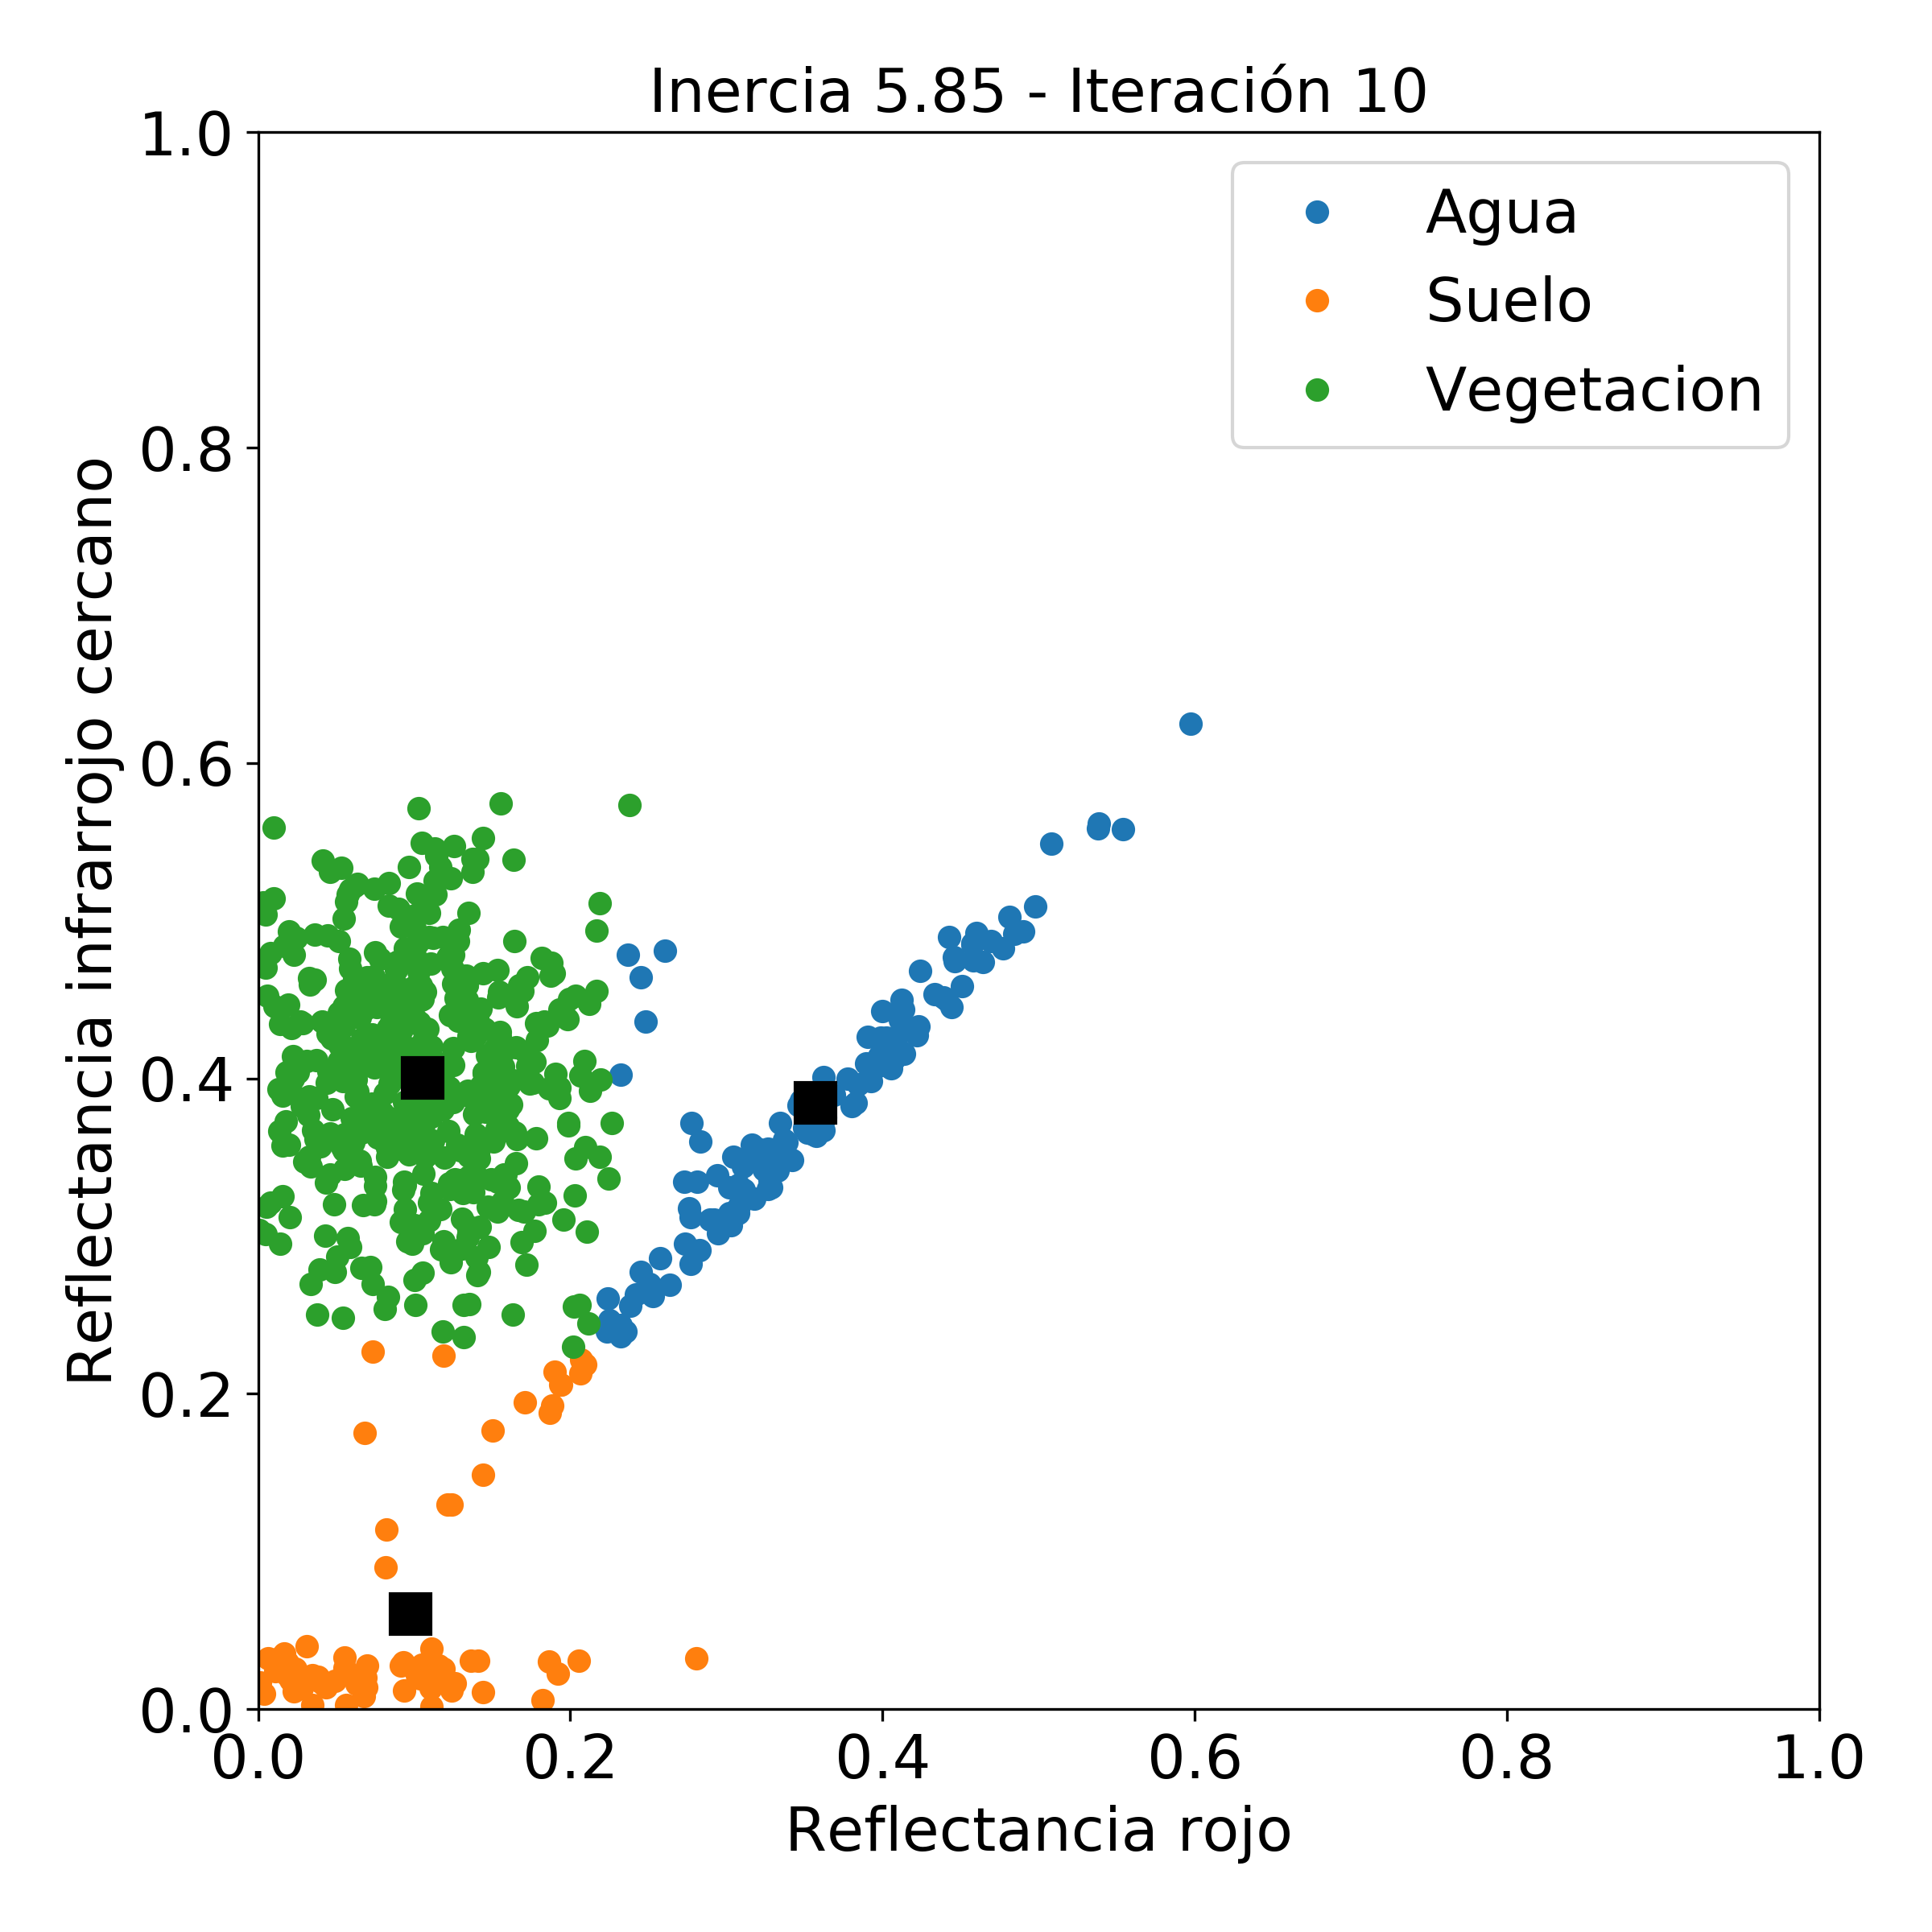
\includegraphics[width=0.4\textwidth]{fig:cluster-10} \label{fig:kmeans1}}
    \caption{Clasificación por kmeans.}
    \label{}
  \end{figure}
\end{frame}
%--- Next Frame ---%




\begin{frame}{\secname : \subsecname}
Muchas gracias.
\end{frame}
%--- Next Frame ---%
